\chapter{Labelling and Symbolization}

\section{Objective of the exercise}
Labelling data and symbolization of data makes it more understandable. In this lesson, the trainees will learn symbolization and labelling of the data.

\section{Data Information}
You will use the following data.
\begin{enumerate}
\item{LocalUnits | Local Units of Nepal | Polygon data}
\item{DIS\textunderscore HQ | District Headquarter | Point data}
\item{MajorRivers | Major Rivers of Nepal | Line data}
\item{Districts | District Boundary | Polygon Data}
\item{RoadNetwork2006 | Road Network | Line data}
\end{enumerate}

\section{Steps}
\subsection{Open ArcMap 10.5}
\subsection{Add data}
\subsection{Labelling}
\begin{enumerate}
\item{Before labelling the data, we need to find the attributes that is stored in the attribute table.Right click on the Districts layer on \emph{Table of Contents} and click Open Attribute Table. Note the attributes and also decide by which value you want to label. For this exercise, we will label the districts by DIST\textunderscore NAME attribute.}
\item{Right click on the DISTRICTS layer in Table of Contents and then click on Properties. A dialogue box appears as shown in figure \ref{fig:properties}} 
	\begin{figure}
	\centering
	\label{fig:properties}
	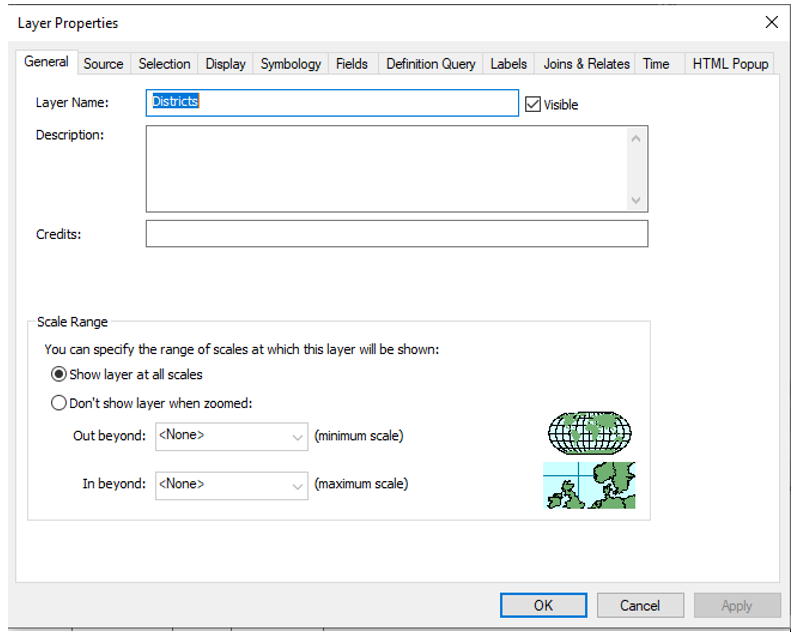
\includegraphics[scale=0.5]{images/properties}
	\caption{Properties Dialogue Box}
	\end{figure}
 
\item{Select Labels. You will see a dialogue box as shown in figure}
	\begin{figure}
	\label{fig:Label Dialogue Box}
	\centering
	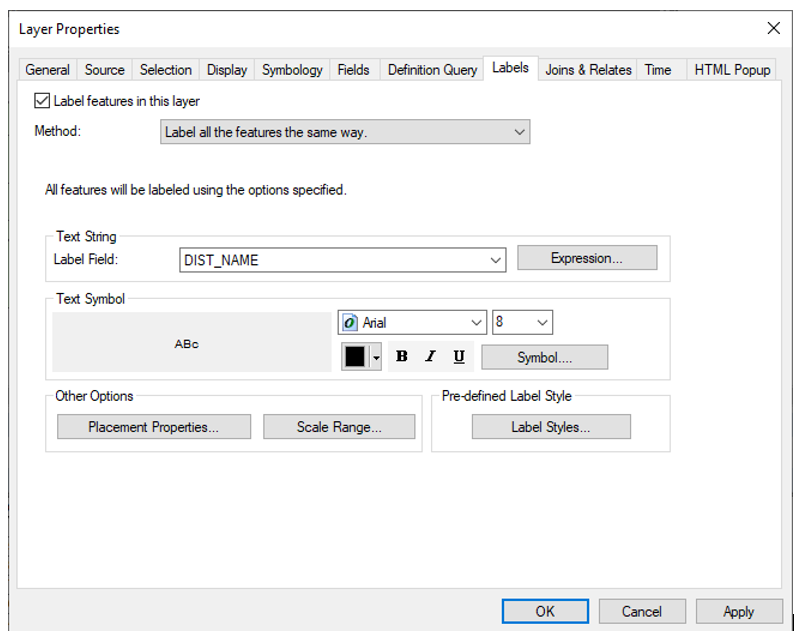
\includegraphics[scale=0.5]{images/label}
	\caption{Label Dialogue Box}
	\end{figure}
 
\item{In the Label Field select DIST\textunderscore NAME. Also tick Label features in this layer as shown in the figure above.}
\item{Click OK. You can see the name of districts labelled above the DISTRICT layer in the map canvas.}

 
\item{Change the color and font sizes of the labels by following the same process.} 

\end{enumerate}

\subsection{Symbolizing the data}
\begin{enumerate}
\item{Just like in case of labelling the data, we need to find the attributes that is stored in the attribute table in order to symbolize the data.}
\item{Right click on the Districts layer in \emph{Table of contents} and click \emph{Open Attribute Table}.}
\item{Note the attributes and also decide by which value you want to label. For this exercise also, we will label the districts by DIST\textunderscore NAME attribute.}
\item{Now right click on the DISTRICTS layer in Table of Contents and then click on Properties.}
\item{Select Symbology}
\item{Select Categories | Unique values. In the Value Field select DIST\textunderscore NAME. Then click Add All Values and click OK. Your symbology should have districts with different colors.}
\end{enumerate}

\subsection{Symbolizing Exercise}
\begin{enumerate}
\item{List the districts of the students in your class. Then, symbolize these districts with red color and other remaining districts with yellow color.}
\end{enumerate}

\subsection{Symbolizing data based on quantity}
\begin{enumerate}
\item{Go to Layer Properties | Symbology. Then select Quantities | Graduated colors}
\item{In the value field, select Shape\textunderscore area.  (Tip : Here, we have classified based on area of each district. Instead, we can also classify based on other attributes such as population, agriculture land, etc. if available in the attribute table).}
\item{Click OK. You can see visualization on map based on the area.}
\end{enumerate}

\subsection{Exercises}
Create a map of Nepal showing the following features:
\begin{itemize}
\item{Districts}
\item{Highways}
\item{District Headquarters}
\end{itemize}
Select appropriate symbology. Label the Districts. 